
\newpage
~
\vspace{30px}

\begin{center}
  \makebox[\textwidth]{
\includegraphics[width=620px]{images/mandelbrot.png}}
\end{center}

\newpage

\section{Problems}

\subsection{The problem of solipsism}

You are aware of your conscious experience.
This knowledge is direct, while the knowledge of the external world is indirect.
The images and sounds which surround you could be something like a dream.\\

{\setlength\parindent{0pt}
\textbf{Solipsist}: The external world does not exist, only subjective conscious experience exists.\\

\textbf{Ray}: In your conscious experience, will the sun rise tomorrow?\\

\textbf{Solipsist}: Probably.\\

\textbf{Ray}: How do you know that?\\

\textbf{Solipsist}: I noticed patterns and created models which describe them. These models describe structures, such as the Sun and the Earth.\\

\textbf{Ray}: So the whole structure is immersed in your subjective conscious experience?\\

\textbf{Solipsist}: Yes.\\

\textbf{Ray}: You might as well say only the structure exists and be done with it. Assuming that it's all immersed in something else is an additional assumption.\\

\textbf{Solipsist}: So what?\\

\textbf{Ray}: Each assumption can be wrong, so the less of them we rely on, the better.\\

\textbf{Solipsist}: I am not convinced.\\

\textbf{Ray}: It is simpler just to have the model.\\

\textbf{Solipsist}: What do you mean by \textit{simplictiy}?\\
}

\newpage

\subsection{The problem of induction}

The sun rises every day but this fact does not logically imply that it will rise tomorrow.
After all, there are phenomena which persist until one day they stop.\\

{\setlength\parindent{0pt}
\textbf{Scientist}: The reason why we predict the sun will rise tomorrow is because our best theories say so.  \\

\textbf{David}: Who is to say our theories will not stop working tomorrow?  \\

\textbf{Scientist}: We reasoned by induction\footnote{The Oxford English Dictionary defines induction as "the process of inferring a general law or principle from the observations of particular instances."} from available data, that's how science works. And it works amazingly well.  \\

\textbf{David}: Who is to say inductive reasoning will not stop working tomorrow?  \\

Answering "induction" would lead to a circualr argument.
This is known as the problem of induction.
Common sense tells us to simply rely on induction, but that does not solve the underlying problem.
}

\newpage

\section{Algorithmic complexity}

\subsection{Strings}

Throughout our life we received a lot of data through our senses from our environment.
The environment is not perceived directly.
What we perceive is our conscious experience.
That experience can be encoded as a string.
Each moment, your visual experience can be encoded as an image with some resolution.\footnote{For example, as a 1MB JPEG.}
The exact algorithm which performs the encoding is irrelevant, as will be explained later.
In any case, the encoding treats time as discrete.
You could encode the visual experience from a series of moments as a series of images.\footnote{For example, you could take an image each 0.1 seconds, or in other words, the images would be sampled with frequency of 10Hz.}
Other senses, or any modality of conscious experience, could be in some way encoded as a string.
Our entire life-experience from the moment we are born until now could be encoded in such a way.\footnote{In reality, we don't have access to such a string. More on that later in the document.}
When we say we observe \texttt{1111}, we mean \textit{we encoded our perceptions as} \texttt{1111}.
A string is a finite sequence of symbols.
Symbols are chosen from a finite set called an alphabet.
Given an alphabet $\{0,1\}$ we can construct a string \texttt{101010}.
That's the alphabet we are going to use for our equations, although the conclusions hold regardless of our choice of alphabet.\footnote{As long as the alphabet is finite and of size $>1$. The explanation of why it makes sense to accept these limitations will be provided later in the document.}
Using an alphabet of $k$ different symbols, there are $k^n$ ways to construct a string of length $n$.
In our examples we will sometimes use the ASCII alphabet, which has 128 symbols, of which 95 are printable.

\newpage

\subsection{Complexity}

Say we observe \texttt{1111} and then stop observing any data.
What kind of a process is generating this data?\footnote{This is equivalent to asking: what is my environment? The environment is wherever the data is coming from.}
It could not be a process which generates just zeroes since that would be inconsistent with the fact that we observed ones.
It could be a process with generates 5 ones and then 5 zeroes.
It could also be a process which generates just a stream of ones without end.
The latter seams a simpler explanation, a simpler theory.
It is also a shorter computer program to write.\footnote{
We have chosen to use some Turing-complete language to describe the members of the set of possible processes.
The alternatives to this will be elaborated later in the document.
Note that we can't use natural language because of the Berry paradox, where we define a natural number as “the least natural number that cannot be described in fewer than twenty words.”
If this number does exist, we have just described it in thirteen words, contradicting its definitional statement.
If such a number does not exist, then all natural numbers can be described in fewer than twenty words.
}
This is the key insight we are going to build upon.
Let's formalize it, step by step.

Take any string $s$ and find a shortest computer program $p$ which generates $s$ as output.
The length of that program $l(p)$ is the algorithmic complexity\footnote{Also known as Kolmogorov complexity.} of $s$, written as $K(s)$.
Our alphabet is finite; if our alphabet were infinite, each program could have its own symbol.
That would make all programs have length 0 or 1.
The program of length 0 is an empty string.

A string $s$ = \texttt{0101010101010101010101010101010101010101} can be generated by the following Python program $p$: \verb|print('01'*20)|.
The length of that program is 14, which, in case it is in fact the shortest program with that output, would give us $K(s) = 14$.
Since $p$ is shorter, we have compressed $s$ into $p$.
This compressions is lossless.
Strings which are easy to compress are simple.
Program length is our measure of complexity.
Another good example of compression is an image of the Mandelbrot set fractal, as the one on the front page of this chapter.
The size of that image is 1.62 megabytes while the program which generates it is very short and takes less than 2 kilobytes to store.\footnote{The code for this is in the github repository: \texttt{code/knowledge/mandelbrot.py}}

To find the shortest program which outputs $s$ we could generate all strings of length 1, length 2, and so on.
Each string we generate, we try to run as a program $p$.
If it's not a valid program we ignore it and go on.
If it does not produce the output which is the same as $s$, we ignore it and go on.
Once we find $p$ with output $o$ where $o = s$, we have our result.
The problem is that when we run some $p$ it can become stuck in an infinite loop.
We can't check for that in advance before we run it.\footnote{
Performing such a check would solve the Halting problem, which is uncomputable.
Is there any other way to compute algorithmic complexity?
It turns out there isn't, algorithmic complexity is uncomputable in general.
}

\newpage

\begin{lstlisting}[caption={Computing the algorithmic complexity of a string. Do not run this at home.}]
import sys
from io import StringIO
import contextlib

def stdoutIO(stdout=None):
	# a function which captures output into a variable
	# the code is in the repo: /code/knowledge/kolmogorov.py

def kolmogorov(s):
	alphabet = [chr(i) for i in xrange(127)] # all ASCII characters
	strings = [[]]
	while True:
		strings = [x + [c] for x in strings for c in alphabet]
		for p in strings:
			try:
				with stdoutIO() as output:
					exec(p)
			except:
				pass
			else:
				if output.getvalue() == s:
					return len(p)
\end{lstlisting}

\newpage

\subsection{Constraint relaxation}

The only way we could compute this if we had a computer which could perform an infinite amount of instructions per second.\footnote{In theoretical computer science, this is known as hypercomputation, or super-Turing computation.}
This implies that infinite loops terminate in 0 seconds.
Nevertheless, this process can be approximated and it can give important conceptual insights.
Some say the only way you can be sure you understand X is when you can write a program which does X.
We can actually separate that into three levels of understanding.
The first level is not being able to write a program for X.
The second level is being able to write it but it works only when run on a computer with infinite speed and infinite memory.
The third level is when your program can run on a real-world computer.\footnote{A problem which can be solved in polynomial time by a bounded-tape Turing machine.}
In order to become capable to solve hard problems first you need to be able to solve simpler problems.
This is similar to physicists trying to solve the problem in ideal conditions before moving on to the realistic case.
This process of simplification, of removing constraints, is crucial to problem solving.

\newpage

\begin{lstlisting}[caption={Approximating algorithmic complexity by limiting the number of instructions $n$ the programs are being executed, as well as the number of different programs which are being executed. As you run this for larger and larger $n$, the return value becomes smaller and smaller, until you reach $K(s)$ and the return value remains $K(s)$ from then on. We say that $K(x)$ is computable in the limit from above. If we were to modify this program so as to put a hard limit on the maximum program length, we could approximate the lower bound of $K(x)$.}]
def exec_one_instruction(p):
	# executes p for just one instruction forward 
	# remembers where it stopped so it can continue from there next time
	...

outputs = {} # partial outputs of all programs we ran so far

def kolmogorov(s, n):
	alphabet = [chr(i) for i in xrange(127)] # all ASCII characters
	strings = [[]]
	while n:
		strings += [x + [c] for x in strings for c in alphabet]
		for p in strings:
			try:
				with stdoutIO() as output:
					exec_one_instruction(p)
			except:
				pass
			else:
				if p in outputs:
					outputs[p] += output.getvalue()
				else:
					outputs[p] = output.getvalue()
				if outputs[p] == s:
					return len(p)
		n -= 1
\end{lstlisting}

\newpage

\subsection{Invariance}

It's not important in which programming language the program is written in or what model of computation\footnote{A model of computation is a model which describes how an output of a mathematical function is computed given an input. Examples: Turing machine, random access machine, lambda calculus...} is chosen, as long as it's Turing-complete.\footnote{This result is known as the invariance theorem for algorithmic complexity.}
Consider a program which is very long when written in C and shorter when written in Python.
We will call the C version $p_C$, the Python version $p_{Python}$, where $l(p_C) > l(p_{Python})$.
Using C we can write a program $compiler_{C,Python}$ which takes Python code as as string input, translates it to C and runs the C code.
Then we can write a new C program which is the same as $compiler_{C,Python}$ but in addition it defines a string variable holding $p_{Python}$ and passes that variable as input to $compiler_{C,Python}$.
Thus the length of the new C program is $l(p_{Python}) + l(compiler_{C,Python})$.\footnote{Technically, we need to add the length of defining a variable in C and calling the function with that variable as an argument. Or we could do it without the variable and pass the string directly.}

We say that a program $p$ which generates $s$ describes $s$.
The shortest such $p$ achieves $K(s)$.
Imagine a plot where on the $x$ axis there are strings, ordered by length and then lexicographically, on the $y$ axis there is $K(s)$.
If we plotted just $K_{Python}(s)$ with an orange line for Python and $K_C(s)$ with a blue line for C, how would that plot look like?
Say we restrict ourselves to those two programming languages and there are no other languages in existence.
For short strings, some may have 2x shorter descriptions in Python, some may be 3x shorter, some may be shorter in C...
Once a certain threshold is passed, the compiler would come into play and the line for $K_C(s)$ would sometimes equal $K_{Python}(s) + l(compiler_{C,Python})$.
Still, some strings, which are best just printed as a literal\footnote{Those are uncompressable strings, this topic will be elaborated later in the document.}, would not require such a compiler at all.

In this simplistic case we are thinking only about two programming languages.
In practice, the program which achieves $K_C(s)$ would use a compiler for some language $X$ which is optimal for the $s$ at hand, not Python. 
This $X$ has both a short program which generates $s$ and also a short compiler written in $C$.
In any case, the speed with which $K_C(s)$ grows is at most as fast as $K_{Python}(s) + l(compiler_{C,Python})$.

There remains a certain arbitrairness when it comes to the choice of a model of computation or a programming language.
Could we somehow compute an average over all programming languages?
Perhaps we could over the first $n$ of them, but in that case the question is how do we start to enumerate them, so we would still be biased.
In the absence of perfection, at least we can take comfort in the fact that the speed with which $K(s)$ grows is the same for every language.

\newpage

\subsection{Terminology}

Which process is generating the data we observed?
The shortest program which generates that data seems like a valid hypothesis.
Also, that program is a potential explanation for what is generating the data.
Every program can be translated to a Turing machine, which means that every program is a mathematical model of what is generating the data.\footnote{Even without translating it to a Turing machine every program can be treated as a mathematical model since everything which can be described at all can also be described by mathematics.}
It is also a theory about what is happening.
In science, the words \textit{theory} and \textit{hypothesis} don't have the same meaning.
Epistemologically, a scientific theory and a scientific hypothesis are both models, the only difference between them is the probability scientists assign to them being true.
Thus, words \textit{process}, \textit{program}, \textit{hypothesis}, \textit{explanation}, \textit{model}, and \textit{theory} are used interchangeably in this chapter.

\newpage

\subsection{Implications}

Is $p$ our theory for what is generating the data?
The problem with using the shortest program $p$ which generates $s$ as an explanation for $s$ is that $p$, after generating $s$, stops.
If science were to use that principle to explain reality, every theory would predict that the world ends at this moment.
We can go around this problem if we do not run the program to its completion.
Instead, while the program is running, we keep track of its output and when we see output identical to $s$ we stop.
In other words, instead of searching for a program which outputs exactly $s$, we search for a program with output which starts with $s$.
This gives us a way to predict future output.
Say we observed data \texttt{1111}, found a program $p$ which starts its output with \texttt{1111}, then we stopped that program.
Say that this program is our theory for what is generating the data which is observed.
We continue running it, one step at a time, until it produces another symbol on the output, and it is a \texttt{1}.
This \texttt{1} is a prediction of our theory about what we will see next.

\newpage

\section{Algorithmic induction}

\subsection{Principle of multiple explanations}

There are infinite possiblities for what generated $s$.\footnote{Say you observe a coin flipped $n$ times, what is the probability that the next flip will result in \textit{heads}? That is, we want to find the bias of the coin. The set of possible hypotheses is uncountably infinite if we allow each real bias in $[0, 1]$, and countably infinite if we allow each rational bias in $[0, 1]$.}
A program is consistent with the data $s$ if its output starts with $s$, otherwise it's inconsistent.
No matter what data we observe, there is an infinity of theories consistent with it.\footnote{"If more than one theory is consistent with the observations, keep all theories." - Epicurus.}
This means that in an ideal case we need to have an infinite amount of theories about what's generating the data, each giving it's own prediction.

Take for example the $s$ = \texttt{1,2,3,4,} what's going to be the next number? The natural answer would be 5. It could also be any other number. The data is consistent with:

\begin{lstlisting}[caption={This gives us 29 as the next number}]
i=1
while 1:
	print(i**4-10*i**3+35*i**2-49*i+24,end=',')
	i+=1
\end{lstlisting}

And with:

\begin{lstlisting}[caption={This gives us 5 as the next number}]
i=1
while 1:
	print(i,end=',')
	i+=1
\end{lstlisting} % this up here has 36 symbols, printing the literal has 10 + len(s) symbols

It is also consistent with \texttt{print('1,2,3,4,')} but just printing the literal string would cease to be the shortest program if for example $s$ = \texttt{1,2,3,4,5,6,7,8,9,10,11,12}.

\newpage

\subsection{Probability}

There are infinite possiblities for what generated $s$.
What are the probabilities?
If you have $n$ consistent theories and $a$ of them predict the next symbol will be \texttt{1} you could say that the probability of seeing \texttt{1} is $a/n$.
This does not take into account the program length.
Take two consistent programs and their binary representations: $p_A =$ \texttt{1010} and $p_B = $\texttt{1010110}.
It seems like $p_A$ is a better explanation, since $p_B$ is just $p_A$ with some bits added to the end.
Still, it is possible for $p_B$ to be a better explanation, it's just less likely.
In the future there could arrive data which make $p_A$ inconsistent and $p_B$ consistent.
If $p_B$ is less likely, how much less?
Since bits can be in 2 states and $p_B$ is longer than $p_A$ by 3 bits, there are $2^{3} = 8$ different ways to add 3 bits to $p_A$ and we chose one of them.
Thus it seems sensible to say $p_B$ is 8 times less likely.
You can think of each added bit as an added assumption, which could be wrong.
Each new element in our explanation reduces probability exponentially. 

To find the probability of next symbol we observe being \texttt{1}, we can generate all programs, for each program $p$ we run it until it produces output $o$ where $l(o) = l(s)$ and see if $o = s$.\footnote{This is uncomputable.}
If $o \neq s$ we discard such $p$ since they are inconsistent.
If $o = s$ then they are consistent.
To each consistent program, using a binary alphabet, we assign a weight of $2^{-l(p)}$.
We go through all consistent programs and run them until they produce next symbol as output.
Each program which outputs \texttt{0} as the next symbol we place in the set $Z$.
Each program which outputs \texttt{1} as the next symbol we place into set $O$.
The ones which terminate without producing output, or end up in infinite loops, we place in set $N$.
The probability of the next symbol we observe being \texttt{1}:

$$\displaystyle P(next=1 \mid s) = \frac{\sum\limits_{p \in O} 2^{-l(p)}}{\sum\limits_{p \in Z \bigcup O \bigcup N} 2^{-l(p)}}$$

This is equivalent to programs voting on what the next symbol is going to be, where each program's vote has weight of $2^{-l(p)}$.
The programs which output \texttt{0} as the next symbol vote for \texttt{0}, the ones which output \texttt{1} as the next symbol vote for \texttt{1}, the ones with no further output vote for $\epsilon$, the empty string.

How could this fail?
It could in the case the sums are infinite, since then the probability is undefined.
Are they infinite?
At the point before we observe any data at all, every program is consistent.
Take all programs of length $x$, there are $2^x$ such programs, each having weight of $2^{-x}$.
The sum of weights for all programs of length $x$ is equal to $2^x * 2^{-x} = 1$.
Our sets contain programs of all lengths.
Both the sum in the numerator and the one in the denominator equal $\infty$, resulting in an undefined probability.

\newpage

\begin{lstlisting}[caption={A naive algorithmic induction implementation, which runs into a problem with infinite sums.}]
alphabet = [chr(i) for i in xrange(127)] # all ASCII characters

def generate_all_programs():
	strings = [[]]
	while True:
		strings += [x + [c] for x in strings for c in alphabet]
	return strings

def exec_until_next_output(p):
	# executes p until it outputs something
	# for each p, remembers where it stopped executing it so it can continue there
	# if p finishes without output, output.getvalue() will return an empty string
	...

def solomonoff(s):
	distribution = {}
	for p in generate_all_programs():
		p_output = ''
		while True:
			try:
				with stdoutIO() as output:
					exec_until_next_output(p)
			except:
				break
			else:
				p_output += output.getvalue()
				if not s.startswith(p_output):
					break
				if len(p_output) == len(s):
					distribution[p] = 2 ** (- len(p))
					break
	return distribution

def probability(outcome, s):
	# outcome: a character
	distribution  = solomonoff(s) # {p: weight,...}
	weights = {character: 0 for character in alphabet}
	for p, weight in distribution.items():
		try:
			with stdoutIO() as output:
				exec_until_next_output(p)
		except:
			pass
		else:
			weights[output.getvalue()] += weight
	return weights
\end{lstlisting}

\newpage

\subsection{Prefix coding} 

When approximating algorithmic induction\footnote{Also known as Solomonoff induction.} we can avoid the problem with infinities by limiting ourselves to only consider programs up to some length $y$.
Yet, if we don't limit ourselves, we get nonsense.
Is there any way around this?

A prefix of a string $s = c_1...c_n$ is a string $s' = c_1...c_m$ where $0 \leq m < n$.
For example, \texttt{0} and \texttt{01} are both a prefix of \texttt{0110}.
Empty string is written as $\epsilon$.
A prefix code is a set of strings $S$ which requires there is no string in $S$ which is a prefix of some other string in $S$.
Take the following binary tree:

\begin{figure}[h]
	\centering
\scalebox{.9}{
	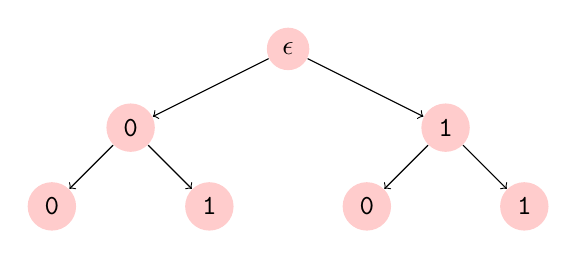
\begin{tikzpicture}
  		[scale=1,auto=left,every node/.style={circle,fill=red!20}]
  		\node (0) at (4,3)  {$\epsilon$};
  		\node (1) at (2,2)  {\texttt{0}};
  		\node (2) at (6,2)  {\texttt{1}};
  		\node (3) at (1,1)  {\texttt{0}};
  		\node (4) at (3,1)  {\texttt{1}};
  		\node (5) at (5,1)  {\texttt{0}};
  		\node (6) at (7,1)  {\texttt{1}};
    	\foreach \from/\to in {0/1,0/2,1/3,1/4,2/5,2/6}
    	\draw[->] (\from) -- (\to);
	\end{tikzpicture}
}
\end{figure}

Take some walk from the root to a leaf, such as $\epsilon \rightarrow 0 \rightarrow 1$.
From such a walk we can construct a string by concatenating the values of the nodes you visit, in this case giving us \texttt{01}.
For every leaf $u$ construct a string $s$ for a walk from root to $u$ and place $s$ in a set $S$.
Since the last character in $s$ is a leaf, $S$ is a prefix code.

For a full binary tree, such as the one shown in the picture, $\sum_{s \in S} 2^{-l(s)} = 1$.
Removing a single leaf which is a child of some node $v$ and constructing a new prefix code $S'$, leads to $\sum_{s \in S'} 2^{-l(s)} < 1$.
Removing another child of $v$, the sum now again equals 1.
In general $\sum_{s \in S} 2^{-l(s)} \leq 1$, where $S$ is a prefix code.\footnote{Known as the Kraft inequality.}

If the set of all programs would form a prefix code, then our sum would not be infinite. 
We can turn an arbitrary set $A$ of strings into a prefix code by transforming each string in a following way, written in Python: \texttt{'1'*len(s)+'0'+s}. 
The set of transformed strings forms set $B$. 
Take a string $s_b \in B$ and its original pair $s_a \in A$, meaning we created $s_b$ by transforming $s_a$ in the way we previously described. 
One way in which some string $x$ could be a prefix of $s_b$ is if $x$ contains only ones. 
Another ways is, $x$ needs to look like \texttt{'1'*len(s\_a)+'0'+q}, where $q$ is some string where $l(q) < l(s_a)$.
Both ways are impossible since $x$ is in $B$.

We generate all programs, transform each program $p$ them into a prefix version $p'$, assign weights on the basis of $l(p')$, before running $p'$ we strip away the leading ones, strip away a zero, this gives us the original program $p$, which we run.\footnote{
This raises a problem of punishing length too harshly, adding a single bit makes the program 4 times less probable.
We can go around that by transforming programs in the way which is described on the next page.
}

\newpage

\begin{lstlisting}[caption={Algorithmic induction with weights being assigned on the basis of a prefix-coded program. Note that nothing is actually being transformed into a prefix string, the only use of it is to assign weights so to guarantee our sum is $\leq 1$. The rest of the functions being referenced in the code snippet here have been introduced a few pages back and they remain unchanged.}]
def bin_str(n):
	# returns an integer n as a binary string, e.g. 5 -> '101'
	return '{0:b}'.format(n)

def transform(s):
	# e.g. 'abcd' -> '1110100abcd'
	# since len('abcd') = 4, which is '100' in binary, len('100') = 3
	# '1' * 3 + '0' + '100' + 'abcd'
	return '1' * len(bin_str(len(s))) + '0' + bin_str(len(s)) + s

def len_of_prefix_string(s):
	bin_len_s = 7 * len(s) # ASCII character can be encoded with 7 bits
	return bin_len_s + 1 + 2 * (floor(log(bin_len_s, 2)) + 1)

def solomonoff(s):
	distribution = {}
	for p in generate_all_programs():
		p_output = ''
		while True:
			try:
				with stdoutIO() as output:
					exec_until_next_output(p)
			except:
				break
			else:
				p_output += output.getvalue()
				if not s.startswith(p_output):
					break
				if len(p_output) == len(s):
					distribution[p] = 2 ** (- len_of_prefix_string(p))
					break
	return distribution
\end{lstlisting}

In this way, the length we added is only $1 + 2 * (\lfloor log_2(l(s)) \rfloor + 1)$.\footnote{For example, adding a signle bit to the $p$ of $l(p) = 10$ makes $p$ 2 times less probable, while adding a single bit to a $p$ of $l(p) = 15$ makes $p$ 4 times less probable.}
As we increase $n = l(p)$, the weights fall in a way which is bounded from below by $f_l(n) = 2^{-n} * 2^{-(1 + 2 * log_2(n) + 2)} = 1 / (2^{n+3} * n^2)$, and above by $f_h(n) = 1 / (2^{n+2} * n^2)$.
Using big O notation, the denominator grows with $O(n^2 * 2^{n})$.

\newpage

\begin{center}
  \makebox[\textwidth]{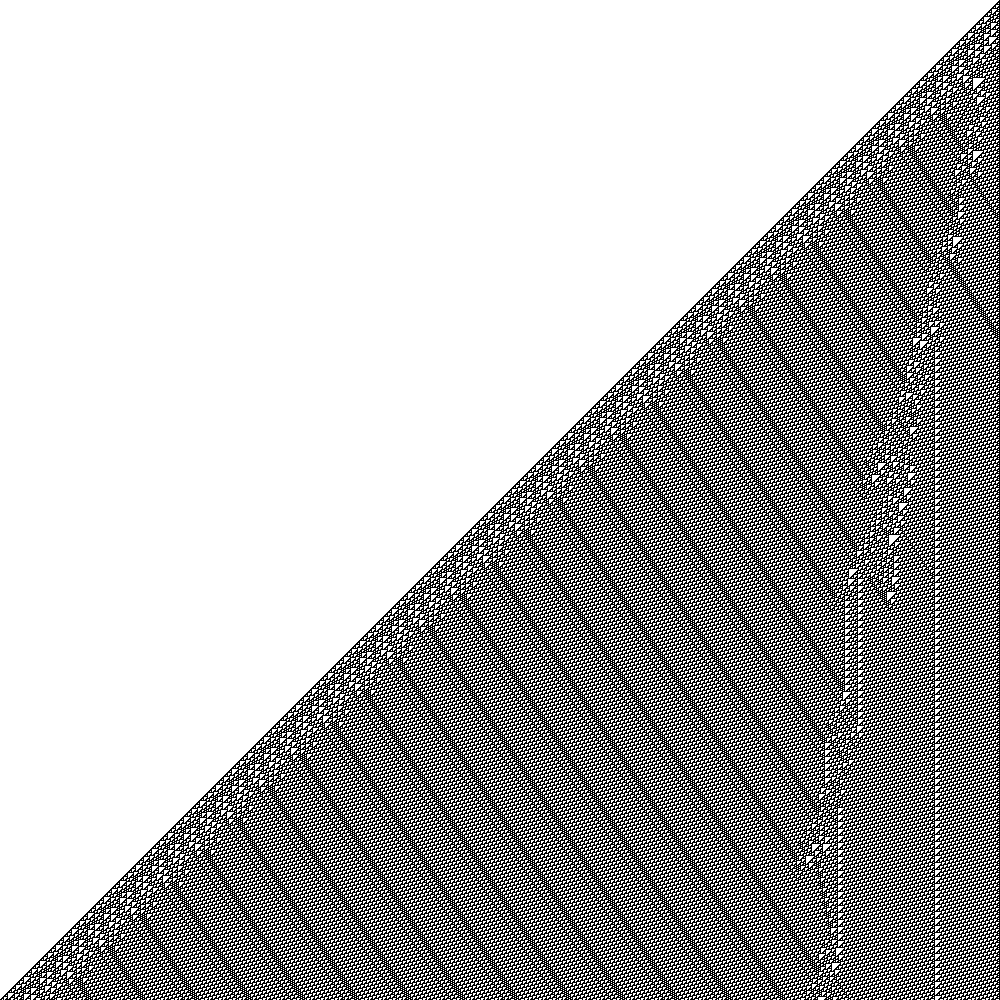
\includegraphics[width=620px]{images/rule110.png}}
\end{center}

\newpage

\subsection{The necessity of data structures}

There are different ways to print output, either print a literal or print some variable.
Are literals good compression?
Literals are not compression at all, it takes more characters to print them than characters in output.
They can't be updated, they always have the same value, while the value of a variable can vary.
Therefore an infinite sequence of updates can be performed on a variable and it can be printed every step of the way.

Let's look at one concrete example of this.
Take a binary string $a$ of length $n$, from it string $b$ of length $n$ can be produced, $b_i$ depending on $a_{i-1}, a_i, a_{i+1}$.
In case $i=0$, we take $a_{i-1} = 0$; in case $i=n-1$ we take $a_{i+1} = 0$.
As an example, here is the \textbf{Rule 110} cellular automaton:

\begin{table}[h!]
\centering
 \begin{tabular}{|c|c|c|c|c|c|c|c|} 
 \hline
 111 & 110 & 101 & 100 & 011 & 010 & 001 & 000 \\ [0.5ex] 
 \hline
 0 & 1 & 1 & 0 & 1 & 1 & 1 & 0 \\ 
 \hline
\end{tabular}
\end{table}

This rule can be summarized as the binary sequence \texttt{01101110}.
Interpreted as a binary number, this corresponds to the decimal value 110, hence the name.
The visual representation of the spacetime of Rule 110 is on the previous page.
The black cells are 1, the white are 0.
The top row is the starting state, the row below that is the next state, etc.
Python code is on next page.

Our data structure, in this example an array, is the equivalent of space.
The need for variables on which to iterate, instead of just printing literals, gives us the loop and thus the equivalent of time.
In case of one-dimensional space, this gives us a nice visual representation of spacetime.

Changing the rule so the 1 becomes a 0 and a 0 becomes a 1 is equivalent, that would be \texttt{10001001}, rule 137.
Also, the rule can be mirrored left to right to produce rule 124.
Changing 0 to 1 and both mirroring left to right produces rule 193.
This is an example of there existing a set of rules which have the same complexity.
In our equations we used a binary alphabet. 
Using an unary alphabet could never achieve a set of rules of the same complexity, since every single program would in that case have a different length.
Additional intuition for why we want to have sets of programs of equivalent complexity is commutativity, $0+1$ is the same as $1+0$.

Say we observe some finite subset of the spacetime.
In that case $p$ needs to have information about the, let's say, upper left and the bottom right cell indexes.
We call this indexical information.

Our program consists of:
\begin{itemize}
\setlength\itemsep{0px}
\item Data structure $u$. Analogous to the \textit{state of the world}.
\item Rules for updating $u$. Analogous to the laws of nature.
\item Encoder which transforms $u$ to output $o$.
\end{itemize}

\newpage

\begin{lstlisting}[caption={A short program implementing Rule 110, together with indexical info. It prints a quite chaotic looking string of length 2500.}]
rule = [0,1,1,1,0,1,1,0]
step = 0 
i = 0
current = [0] * 99 + [1]
successor = []
total = []
while step < 100:
	total.append(current)
	while i < 100:
		left = 0 if i == 0 else current[i-1]
		mid = current[0]
		right = 0 if i == 99 else current[i+1]
		successor.append(rule[4*left + 2*mid + right])
		i += 1
	current = successor
	successor = []
	i = 0
	step += 1

i1, j1, i2, j2 = 50, 50, 100, 100 # indexical info
for i in range(i1, i2):
	for j in range(j1, j2):
		print(total[i][j],end='') # encoding
\end{lstlisting}

\begin{lstlisting}[caption={A short program generating an infinite universe of Rule 110. The question of how indexical information works in an infinite universe is addressed later in the document.}]
rule, i, x, current, successor, total = [0,1,1,1,0,1,1,0], 0, 0, [], [], []
while 1: current.append(0)
while 1:
	total.append(current)
	while 1:
		successor.append(rule[4*x + 2*current[i] + current[i+1]])
		i, x = i + 1, current[i]
	current, successor, i, x = successor, [], 0, 0
\end{lstlisting}

\newpage

\subsection{Incompressibilty}

The probability of the shortest program can still be very small if there is a sufficient number of sufficiently probable consistent longer programs.
As length increases, the probability of the programs decreases exponentially, but the number of them also increases exponentially.
It is possible that the shortest program will have an astronomically small probability.
Intuitively, a large majority of those longer programs would have refutable components. 
There are various ways to take a short program $p$ and create an equivalent longer program $p'$: add comments, rename variables and functions, assign values to variables which do nothing, etc.\footnote{
We say the programs are equivalent if they, when executed, instantiate identical data structures.
As an example, take a programming language with alphabet $\{1,\#,\alpha\}$, where \# stands for beginning of a comment, $\alpha$ stands for newline.
Now take a program $p$ with 2 lines of code: $\#\alpha\#\alpha$.
It has a length of 4 and weight of $3^{-4}$.
This program doesn't do anything, but the content on the lines before the \# sign are irrelevant, they could've been anything.
Focusing only on 2-liners, here are the equivalent programs of length 5: $\{\#\#\alpha\#\alpha, \#\alpha\#\#\alpha, \#1\alpha\#\alpha, \#\alpha\#1\alpha\}$.
The sum of their weights is $4 * 3^{-5}$, which is by a factor of $4/3$ more than our $p$.
This looks like trouble but does not hold in general, looking at 2-liner equivalents of $p$ of length $4+k$, there are $2^k(k+1)$ of them.
There are 2 characters which can be used to form the text of the comments.
Once a text of length $n$ is produced, it can be split in $k+1$ ways so that one part of the string goes on the end of the first line, the other part goes at the end of the second line.
Each such equivalent has a weight of $3^{-k}$.
Total weight of all equivalents of length $>4$ is $\sum_{k=1}^{\infty} (2/3)^k(k+1) = 9$, which is $3^6 = 729$ times more than the weight of the shortest program $p$.
We could also put $p$ and all those $p$-equivalent programs in an equivalence class, where the weight of such class is the sum of the weights of programs which are members of it.
Then we can compare such classes against one another.
}

Denote a set of all programs of length $n$ which are consistent with $s$ as $X_n$.
As $n$ increases, does the probability mass of $X_n$ decrease?
In our example it did (except for $k=1$), but does it behave in such way in general?
There are $2^n$ binary strings of length $n$, and $2^n-1$ binary strings of length $<n$.
Therefore there is at least one n-bit string that does not have a consistent program of length $<n$.
There are $2^{n-c}-1$ binary strings of length $<n-c$.
The chance for some random string of length $n$ to have a consistent program of length $<n-c$ is at most $(2^{n-c}-1)/2^n$ which is less than $2^{-c}$.
Most strings are very incompressible.

Take a set of programs with length $<n$, call it $S_n$.
When $n$ is very small, there will perhaps be no programs in $S_n$ consistent with $s$.
As $n$ increases, at some point say there will be one program in $S_n$ consistent with $s$.
Now consider $S_{n+1}$, which contains 2 times more programs.
Are there now also 2 programs consistent with $s$ in $S_{n+1}$?
Take a set of all strings $s$ which are consistent with some program in $S_n$, call that set $C_n$.
Assume we find that for each $s \in C_n$ there are twice the number of programs consistent with $s$ in $S_{n+1}$ than in $S_n$.
That would imply that $C_n = C_{n+1}$, which is false, because $C_{n+1}$ will contain some strings which were incompressible for $n$, i.e. there were no programs consistent with those strings in $S_n$.
As $n$ increases, the ratio $|X_n|/|S_n|$ decreases and the total probability mass of $X_n$ also decreases.
Hence, from now on we will mostly focus on our shortest consistent program $p$ and its properties.

\newpage

\section{Implications for epistemology}

\subsection{The problem of induction dissolves}

What was our goal?
We arrived at a particular program by trying to explain the existing data we have already seen.
What is the fruit of our solution?
That program also gives us predictions.
The programs which behave according to the same principles all the time are shorter than programs which produce data according to one set of rules for some time and then change and start producing data according to some other set of rules.\footnote{
The universe which behaves one way and then just stops would need to know when to stop.
That requires a constant to be defined, which makes such a program longer and less probable.
Planck time is approximately $5.39 * 10^{−44}$ seconds.
The age of the universe is around 13.8 billion years.
This gives us around $8.07 * 10^{60}$ Planck time units.
Some program could for example stop at step \texttt{10**61}.
The longer the time goes on, such round numbers become exponentially less frequent.
}

\begin{lstlisting}[caption={A short program using one rule for the first 100 time steps, another rule from then on. This program is longer than just using the same rule all the time.}]
rule1, rule2, i, x, current, successor, total, k = [0,1,1,1,0,1,1,0], [1,0,0,0,1,0,0,1], 0, 0, [], [], [], 0
while 1: current.append(0)
while 1:
	total.append(current)
	while 1:
		rule = rule1 if k < 100 else rule2
		successor.append(rule[4*x + 2*current[i] + current[i+1]])
		i, x = i + 1, current[i]
	current, successor, i, x = successor, [], 0, 0
\end{lstlisting}

This is why the sun will very probably rise tomorrow.
The problem of induction dissolves.
Our knowledge enables us, to a limited degree, to see into the future.

\newpage

\subsection{Solipsism dissolves}

How would a solipsistic program look like?
It would look like your mind is the whole universe.
The solipsist's view is that not only is there a program $p$ which describes what is happening, but also that $p$ is running inside his mind.
This new program includes both $p$ and wraps its internal data structure $u$ in a larger structure, where the larger structure does not influece the output in any way.
This explanation is more complex than just specifying a shortest program which outputs the data which is consistent with observations. 

\begin{lstlisting}[caption={A solipsistic program.}]
rule, i, x, current, successor, total = [0,1,1,1,0,1,1,0], 0, 0, [], [], []
while 1: current.append(0)
while 1:
	total.append(current)
	while 1:
		successor.append(rule[4*x + 2*current[i] + current[i+1]])
		i, x = i + 1, current[i]
	current, successor, i, x = successor, [], 0, 0
mind = [total]
\end{lstlisting}

Solipsism is similar to the hypothesis that we are living in a simulation.
This, however, does not show that the chance we are living in a simulation is low.
Neither does it show that there is a low \textit{prior} probability of us living in a simulation.
In case some agent investigates the laws of physics and finds them very complex, algorithmic induction could show that it is more likely that he is embedded in a simulation being run inside a simpler outer universe.
Of course, that outer universe needs to contain a simulation of the inner universe the agent is embedded in.
It could be a shorter program overall.\footnote{This will be more clear after the \textit{1.6.2 Indexicality} subsection.}

\newpage

\subsection{The problem of other minds dissolves}

You are aware of your own thoughts and experiences but not aware of other peoples' experiences.
It is entirely consistent to suppose other people don't have them.
Such entities, which lack consciousness but behave the same as people who have consciousness, are known as philosophical zombies.
How would a program in which only one human is conscious look like?

\begin{lstlisting}[caption={A zombie-filled program.}]
spawn_conscious_agent()
while 1:
	spawn_zombie()
\end{lstlisting}

\begin{lstlisting}[caption={A more probable program.}]
while 1:
	spawn_conscious_agent()
\end{lstlisting}

However complex of a phenomena consciousness is, the process which generates consciousness in you is probably present in other people as well.
It is a simpler explanation than that of you having an unique process which creates consciousness uniquely in you.
Whatever consciousness is, the program which gives rise to consciousness in all humans is simpler than the one in which you need to additionally specify which specific human is conscious.

\newpage

\subsection{Supernatural explanations dissolve}

Why did it rain?
It could be some wizard caused it by casting a spell.
How would a program in which supernatural entities exist look like?
A DNA sequence is just a part of a definition of an organism, since it's the interaction between the prenatal environment and the DNA which actually constructs the organism.
How long is God's DNA?
Supernatural entities such as wizards, demons, and so on, are all complex objects consisting of a large number of parts, while the mechanisms which actually cause rain can be defined with a few equations.

\newpage

\subsection{The relationship to the Bayes' theorem}

To each program we distributed a weight.
Is the weight distribution a probability distribution?
As we observe more data, more of our programs become inconsistent and hence eliminated.
The sum of all weights of consistent programs is falling as the length of $s$ increases.
Thus, the weight distribution is not a probability distribution because the sum of all weights is not 1.
In order to turn it into a probability distribution each weight needs to be divided by the sum of all weights.\footnote{In words of probability theory, it needs to be normalized.}
Before observing any data, all programs are consistent, and we start with the \textit{prior} probability distribution.
The hypothesis that program $p$ is generating $s$ we write as $H_{p}$.
There are two cases, $p$ outputted \texttt{1} as the next symbol or $p$ outputted \texttt{0} as the next symbol.\footnote{
As before, all $p$ which output $0$ as the next symbol we place in set $Z$, ones which output $1$ as the next symbol we place in $O$, the ones which get stuck in infinite loops or terminate without further output we place in $N$.}
Now we observe $E =$ \texttt{0} and perform a Bayesian update.

$$ P(H_{p} \mid E) = \frac{P(E \mid H_{p}) P(H_{p})}{\sum\limits_{p \in Z \bigcup O \bigcup N} P(E \mid H_p) P(H_p)} $$

\vspace{15px}

\textbf{In case $p$ outputed \texttt{1}}, $P(E \mid H_{p}) = 0$, which gives $P(H_{p} \mid E) = 0$.
Once a hypothesis has probability zero, meaning $P(H_p) = 0$, following the Bayes' theorem it can't be updated to any other probability.
This is equivalent to eliminating all programs which are inconsistent, their probability is $0$.

\vspace{15px}

\textbf{In case $p$ outputed \texttt{0}}, $P(E \mid H_{p}) = 1$.
The denominator sum can also be simplified since $P(E \mid H_{p}) = 0$ for all $p$ in $O \bigcup N$, which gives us:

$$ P(H_{p} \mid E) = \frac{P(H_{p})}{\sum\limits_{p \in Z } P(H_p)} $$

This is equivalent to renormalizing the weights for all programs which are consistent, which gives us probabilities.
Our theory is equivalent to the Bayes' theorem where the prior is based on program length.

\newpage

\subsection{Priors}

Note that the data by itself tells us little.
We started with an infinite number of possible theories and we remained with an infinite number of possible theories, only some of them got eliminated.
Among the ones which did not get eliminated, what is the probability distribution?
That question is answered with a theory, not data.
Everything is dependent on the prior.

Consider a situation in which one knows a ball has been hidden under one of three cups, \texttt{A}, \texttt{B}, or \texttt{C}, but no other information is available about its location. 
In this case a uniform prior of $p(A) = p(B) = p(C) = 1/3$ seems intuitively like the only reasonable choice. 
We can see that the problem remains the same if we swap around the labels (\texttt{A}, \texttt{B} and \texttt{C}) of the cups. 
It would therefore be odd to choose a prior for which a permutation of the labels would cause a change in our predictions about which cup the ball will be found under.
The uniform prior is the only one which preserves this invariance. 
If one accepts this invariance principle then one can see that the uniform prior is the logically correct prior to represent this state of knowledge. 
The prior is not an observer-independent feature of the world.
In reality the ball exists under a particular cup, and it only makes sense to speak of probabilities if there is an observer with limited knowledge about the system.\footnote{
The Shannon entropy of a probability distribution measures the amount of information contained in the distribution.
The larger the entropy, the less information is provided by the distribution. 
The distribution which maximizes entropy is the least informative.
For example, the maximum entropy prior on a discrete space is the prior that assigns equal probability to each state.
This is known as the principle of indifference or the principle of insufficient reason.
This principle is subject to Bertrand'd paradox, which will be addressed in later chapters.
}

In case where we have a finite number of options, the choice of the prior seems clear.
What if we had an infinite number of options?
In case of algorithmic induction, instead of an uniform prior, we based our prior on the program length.
If instead we were to use an uniform prior, the probability of every single program would be 0.

\newpage

\section{Implications for philosophy of science}

\subsection{Science is both prediction and explanation}

Science can be viewed as an approximation of algorithmic induction.
Scientists search for theories which are consistent with the data.
They use criteria which they call elegance, simplicity, and Occam's razor\footnote{“It is vain to do with more what can be done with fewer.” - William of Ockham}, which are equivalent to preferring shorter programs.
Each program is equivalent to an explanation of how the world works.
Their theories also make predictions.
The goal of science is not \textit{only} prediction, nor is it \textit{only} explaining the world, it is both.
For each set of laws of physics, you can create a virtual reality environment inside of which those laws hold true.
All virtual realities which behave the same as our world are explanations of how our world works, with the simpler ones being more probable.

\newpage

\subsection{Explanatory power is compression rate}

How many programs are there in science today?
We still do not have a single theory which explains everything.
We have multiple theories which each compress certain subsets of the data we observed.
Is their compression lossless?
Our theories do not compress the data perfectly, but approximately, their compression is lossy.
The first reason why they are lossy is an imperfection in the theory, such as Newton's theory being a lossy compression in comparison to Einstein's theory.
The theories of the future will increase our resolution further.
The second reason is an imperfection in the data due to measurement error.
A program which compresses our astronomical data perfectly would need to take into account the way in which the data was gathered, and in such process transformed, by our telescopes, errors included.
The third reason is because the domain of the problem is purposefully reduced for practical reasons, so it can be easier to attack and solve the problem at hand.
To model something complex it's often useful to first model a simplified version of it.\footnote{Also, there is a tradeoff between \textit{making the model more complex and more prone to overfitting} on the one side, and \textit{making the model simpler but increasing the error of the hypothesis} on the other.}

Theories which explain a lot of different phenomena at the same time while being simple are said to have greater explanatory power.
That is because they have greater rate of compression, which would be the length of data divided by the length of the program.
Hence, explanatory power is directly proportional to probability.

As we gather more knowledge the rate of compression increases as we unify models such as when light, electricity and magnetism were merged into electromagnetism, or when heat was understood to be the motion of atoms, or when Einstein connected geometry and gravity.
If this progression of knowledge continues, one day we may know everything there is to know.\footnote{At least when it comes to theoretical knowledge.}
We could have a theory of everything.
Once we have the theory, further improvements to the theory could be made by unifying different fields of knowledge, or in other words, compressing it further.

\newpage

\subsection{Ockham and memory}

The stars are actually other suns, operating according to the same laws as our sun does.
There are billions and billions of them.
Wouldn't the world be simpler if instead of all those suns we had just a single glass sphere surrounding the Earth, with holes through which the light from outside would enter?
This is exactly what William of Ockham meant when he said that \textit{entities} are not to be multiplied beyond necessity.
In saying that he got it exactly wrong.
It is not entities which should not be multiplied, it's the laws.
How much memory does our program have available?
The universe seems like it has limitless memory capacity.
Memory is cheap while the descriptions are expensive.

\newpage

\subsection{Infinite space}

With every new symbol of $s$ we observe, i.e. with every new bit of information we receive, our probability distribution over the set of programs changes.
Therefore, our predictions change with each new bit of information we receive.

On the basis of an extinct animal's fossil, by the shape of its teeth, we can conclude if the animal was a herbivore or a carnivore.
The evidence is indirect, as all evidence is, the evidence for the theory being true is always gathered from the effects of that theory being true.
In the case the theory wasn't true, the world would look differently than it does.
Even when reading a chemistry textbook you believe the textbook without performing every experiment yourself.
If the results of experiments were different, then the textbook would be written differently.
When viewing the world with your eyes, you are not looking at the objects directly but you are observing the effects which reflected light has on your nerves.
Every piece of evidence is indirect.
Thus, existence of invisible things can be deduced from their effects on the visible things, for example, the existence of dark matter and dark energy.

Can we know that our universe is infinite?
The best model in cosmology today is a model in which the universe is infinite.
If it was finite then the cosmic microwave background radiation would look differently than it actually does.
The shortest program which is consistent with the data uses equations in which the space is infinite.
The data we see reveals us something about the data we do not see because that unseen data is too far in space.
This is not surprising, since the data we see also reveals us something about the data we do not see because the unseen data is too far in time, namely, in the future.
Our theories tell us about things which are far in spacetime.

\newpage

\subsection{Short programs are refutable}

Any program consistent with the data can be changed by adding some useless parts which make the program longer but do not alter the output.
The predictions of both programs are the same, so this additional parts can't be ruled out as false, those parts are irrefutable.\footnote{
The concept of refutability is unfortunately also known as falsifiability.
That term is clumsy, when someone talks about falsification, what first comes to mind is the usual definition of fraud and forgery, falsification of records.
}
The only way to produce irrefutability is by making the explanation longer than it needs to be.

It may appear that the theory which claims the universe is infinite is irrefutable, since we can't actually visit all of the universe and thus confirm it is infinite.
In fact it is refutable because it does make testable predictions about cosmic radiation.
You do not need to be able to go to the end of space and personally check if it is infinite.
The theory of an infinite universe is the shortest program which compresses the data and as such of course it is refutable.
Good explanations, same as good algorithms or stories, are hard to vary\footnote{Expression taken from David Deutsch.}, because every part plays an important role.\footnote{As Wittgenstein says, a wheel that can be turned though nothing else moves with it is not part of the mechanism.}
Even though theories can have irrefutable parts, taken as a whole, every theory is refutable, since every theory makes predictions.

\newpage

\subsection{The way we compute is the way things are}

Our observations of the planetary motion are consistent with a geocentric model of the solar system.
Is heliocentrism just a simpler way to compute?
In order for geocentrism to make correct predictions it needs to model planetary motion as circles within circles, which leads to a longer description of the laws of nature.
You could claim that the heliocentric system is just a simpler way of computing things while in reality the Earth stands still.
That would certainly be more intuitive to accept, the Earth looks like it is standing still.
The Earth also looks like it is flat.
If it's round, does that mean that the people on the other side stand on their heads?
It turns out that concepts of up and down are not fundamental but are defined in relation to the center of the Earth as explained by the law of gravity.
The Earth also looks exactly like it is round with a curvature of around 8 cm per kilometer and moving around the Sun with speed of 30 kilometers per second.
The fact you don't feel the movement is because there is no acceleration.
Today we learn this facts in school as children and grow to accept them as obvious.
They are not obvious at all, they are shocking, and if we didn't learn them as children they would be much less widely accepted.
It is not clear at first sight that we should accept them only because they are the simplest way to explain the data.
Our preference for simpler explanations is a crucial principle by which we form our view of the world.
The progress of science continually runs counter to our intuitions, which is exactly what you would expect from the fact that we are evolved creatures, our intuitions evolved to understand the world at a scale from roughly $10^{-4}$ to $10^7$ meters.
This is why when it comes to scientific questions our inborn intuitions can be ignored.\footnote{
This does not imply intuition can be ignored in your personal life.
Also, the intuitions of a professional scientist, mathematician or an engineer are developed over time with practice and are often the reverse from the natural intuitions one is born with.
}

\newpage

\subsection{Improved theories will be consistent with old ones}

Are our best theories correct?
Heliocentrism could still be wrong.
We used to think the Earth to be flat, then to be a sphere, then to be a sphere which is slightly flattened at the poles, then we concluded it has an irregular shape called a geoid.\footnote{Idea from \textit{The Relativity of Wrong} By Isaac Asimov.}
Science seems to change its mind a lot.
Yet each correction was smaller than the previous one, our models becoming less and less wrong.
The simple version of heliocentrism in which the Earth rotates around the Sun is in fact wrong.
The Earth rotates around the solar system's center of mass, which is never perfectly in the center of the Sun, it's tilted slightly, mostly affected by Jupiter.
When we discover the theory of everything we can be sure it will be consistent with this updated version of heliocentrism.

\newpage

\section{Subjectivity}

\subsection{Encoding}

We started by encoding our sensory data as a string.
How is that encoding performed?
We could separate our visual field into some number of pixels, each pixel having 3 components (for red, green and blue), every component having values from 0 to 255.
Is the pixel \texttt{(0, 0, 0)} black or white?
Or, what if we choose to use \texttt{CMYK} values?
What if we choose some other resolution?
Or a different sampling rate?
A similar question: is my red the same as your red, or do you perceive red as I perceive blue?
In the ideal situation, every agent would use the same encoding.
Unfortunately, this can't possibly be guaranteed.

As we saw in our cellular automaton example, one component of our program $p$ is the data structure $u_p$.
At a certain point in time our $u_p$ is in state $u_{(p,n)}$, at a next it is in state $u_{(p,n+1)}$, and so on, $u_{p}$ being a totally ordered set $\{u_{(p,0)},u_{(p,1)}...\}$.
Another component are the rules which update the data structure from state $u_{(p,n)}$ to $u_{(p,n+1)}$.
What we will call an engine is the union of the data structure and the rules.
Another component is the encoder $e_p$, which takes $u_{(p,n)}$ as input and translates it into a string $o_{(p,n)}$, written as $e_p(u_{(p,n)}) = o_{(p,n)}$.\footnote{Technically, it can take any subset of $u_p$ and map it, but it's easier to talk about it in this way.}
The total output $o_p$ of $p$ is equal to $s_p = o_{(p,0)}...o_{(p,m)}$.
In case we choose to encode our sensory data as \texttt{RGB}, there exists a $p$ which also encodes $u$ as as \texttt{RGB}.
If we chose \texttt{CMYK}, there exists some other $p$ with the same engine but $e_p$ uses \texttt{CMYK}.
Whatever we chose as an encoder for our sensory data, the shortest program which is consistent with the data will have the same encoder, because otherwise $p$ would not be consistent with the data.

Can the choice of encoding influence what will be the engine of the shortest program?
Some data structures are easier to encode as \texttt{RGB}, some harder.
Thus, it is possible that it will.
For each possible encoding $e_i$ find the shortest consistent program $p_i$.
Is there a bijection between $u_{(p_i,n)}$ and $u_{(p_j,n)}$?
Take an example of run-length encoding, \texttt{AAAAABBAAAAAAA} being encoded as \texttt{A5B2A7}.
There is a bijection between them because one is a lossless compression of the other.
Take a program which generates Rule 110 cellular automaton and has an encoding $e(0)=1; e(1)=0$.
This is the same as a program which generates Rule 137\footnote{Which is the same as Rule 110 but \textit{flipped} so 0 is 1 and 1 is 0.} and has an encoding $e(0)=0; e(1)=1$.
There is a bijection between states of Rule 110 and Rule 137.
If there were no bijection that would imply that some $u_{(p_i,n)}$ does not contain the same information as some other $u_{(p_j,n)}$.
That is expected when one encoding contains more information than the other, because of higher resolution or sampling rate.
As an example of loss of information, take an encoding of a state in Rule 110 which maps, for example, the state \texttt{0010} to \texttt{01}, and state \texttt{0011} also to \texttt{01}.
In case there is a bijection between $o_{(p_i,n)}$ and $o_{(p_j,n)}$, there should be a bijection between $u_{(p_i,n)}$ and $u_{(p_j,n)}$.
The nonexistance of such a bijection that would imply the existence some data in $u_{(p_i,n)}$ which has no effect on output and is different from the one in $u_{(p_j,n)}$.
That seems unexpected considering $p$ is the shortest consistent program.
Even if two agents choose different encodings, the engines of their programs shoud be equivalent.

\newpage

\subsection{Indexicality}

If one agent observes $s$ which starts with \texttt{1}, another observes $s$ which starts with \texttt{0}, they will never have the same theory.
In general, the strings of different agents will be different, because the agents are instantiated at different points in spacetime, which means different programs will be consistent with their strings.
How would the program which outputs your life look like?
It would look different than the one which outputs some other agents' life.
It would be easier if every agent converged on the same $p$.
Unfortunately, this can't possibly be guaranteed.

As we saw in our cellular automaton example, our encoder $e_p$ needs to have indexical info, about where you were in time and space for your whole lifespan.
This is not a problem for finite universes, but it would be ideal for a theory to work both in finite and infinite universes.
In an infinite universe, this info is infinite.\footnote{Even in a large finite universe, $l(info)$ can be larger than just hardcoding $s$ as output $o$.}
What if we change our induction algorithm by not requiring the output $o$ of our program $p$ to be identical to $s$, but only requiring that $o$ contains $s$?
This does not seem like a good solution, since a $p_\pi$ which generates $\pi$ is very short and its $o$ also contains $s$.

Indexical info can be a string $s_\delta$ which is a substring of $s$.
For example, $s_\delta$ could be the last minute of the agents' lifespan.
Then $p$ searches $u$ through space and time, sampling all possible subsets of it and encoding them, until it finds some subset of $u$ which when encoded gives $s_\delta$.
Once it finds it, it has located the agent which is embedded in $u$, and from then it should be possible to keep locating the agent back through time.
How exactly is the rest of $s$ printed is at this point not clear, but it may depend on some pattern recognition algorithm.\footnote{More on that in some later chapter of the document.}
If humans could in principle do it, then some program should be able to do is as well.
When $len(s_\delta) << len(s)$, that kind of program could be the shortest program which outputs $s$.
The subset of $u$ which when encoded gives $s$ we can call $u_\lambda$, it is the preimage of $o$ and $s$.
There could be many different subsets of timespace which, when encoded, give $s$.
In an infinite universe there could be an infinite amount of them.
Which of those we choose to encode depends on the search algorithm of the shortest consistent program.\footnote{
It may seem like the shortest program $p$ which is consistent with the data we see is the one which generates all possible universes, and contains indexical info.
That would assume that our indexical info $s_\delta$ is enough to pick out some subset of $u$ using which we can recreate complete $s$ correctly.
This is extremely unlikely to happen by chance, in order for that to happen our search algorithm would need to know where to search.
}
Shorter the search algorithm, the better.
Given the same encoding, agents with different indexical info should converge to the same engine.

\newpage

\subsection{Reality}

I think, therefore I am...  an agent which is performing some kind of computation and as such I am embedded in an universe which supports computation.
The agent is embedded in the data structure $u$, only a part of which is, due to indexicality, being printed by $p$.
That data structure is our \textit{universe}.
The structure has effects on the programs' output, and therefore on our input.
That which has effects on what we see is called \textit{reality}.

Choice of the programming language\footnote{Or more generally, of the model of computation.}, of encoding and the location of the observer all change $p$.
Run algorithmic induction with choice of programming language $L_1$, encoding $E_1$, and the agent being instantiated in some spacetime location $I_1$.
The shortest program will be $p_1$.
Now run it for $L_2$, $E_2$, $I_2$, and the shortest program will be some other $p_2$.
There is no equivalency between program and the model of reality.
Reality is a structure which is preserved through the space of different languages, encodings and locations.
One instantiation of that structure is the programs' engine.
Our terminology needs to be updated, there is an equivalency between the words: \textit{engine}, \textit{process}, \textit{hypothesis}, \textit{explanation}, \textit{model}, and \textit{theory}.
Since each program has a corresponding engine, we can still use the word \textit{program} to refer to the engine.
We are using program length to measure the complexity of the engine.

The agent can never have a full model of the world since it needs to model itself as a part of the world, which means the model of the world needs to be a compressed low-resolution representation of the world-state.
There is no knowledge, only a probability distribution on models.
What we usually call knowledge are just models we are very certain of.

\newpage

\subsection{Observation selection problem}

An observation selection effect exists when some property of a thing is correlated with the observer existing in the first place.\footnote{\url{https://wiki.lesswrong.com/wiki/Observation_selection_effect}}
An agent can ignore all programs which are not complex enough to contain bounded-tape Turing machines within them, or something equivalent to them.
To perform this pre-filtering the agent would need to be able to prove, for any program $p$, are the rules which generate $u$ Turing-complete or not?
In other words, by controlling the intial state of the universe, could we represent any possible computer program?\footnote{That would also imply that by reading some later state of the universe you can retrieve the result of that computation.}
Ordinary algorithmic induction, used in this chapter so far, performs no such pre-filtering.
It just generates all programs which are consistent with the data, including programs which have rules which are not Turing-complete.

Consider two universes $A$ and $B$.\footnote{To simplify, we can assume $l(A) = l(B)$.}
Say the universe $A$ contains ten agents which are identical to us, while the universe $B$ contains only one such agent.
It seems reasonable that $A$ should have ten times greater prior probability of being the one in which we are embedded.
The finite case is clear, but in case the universes are infinite, there may be an infinite number of agents in each universe.
Still, in some universes $u_\lambda$ may appear more frequently than in other universes.
According to our current theory, this density of $u_\lambda$-patterns within $u$ makes no effect on the probability of $p$.

\newpage

\section{Metaphysics}

\subsection{Time}

Up until now, we viewed $u$ from the outside perspective, we had maintained a view from nowhere.
There was $u$ and some part of $u$ was deemed to be \textit{observed}, and the value of those observations was stored in some platonic string $s$.
This perspective felt natural because the algorithm which we are talking about requires infinite memory and as such can only be analyzed from the platonic perspective.
It's something the agent can never run, it can only run approximations of it.

The sting $s$ is a product of encoding subjective conscious experience.
This process of encoding is required if we wish to apply the theory to humans, but can digital agents receive $s$ directly from the input?
Not exactly.
The input $s_0$ which the digital agent receives from the environment is transformed by its internal processes and forms some organized internal structure.
This structure is equivalent to conscious experience, and is then somehow encoded and \textit{sent}\footnote{This is impossible, but that's the view from nowhere.} as an input $s$ to algorithmic induction.
Induction finds the shortest program, which instantiates a universe $u$ and maps a subset of it to $s$, meaning it maps the equivalent of \textit{positions of quarks} to $s$.

The only thing we are aware of is the current moment.
We have no direct experience of the past, our awareness knows just the few past seconds.
Our starting point is our direct conscious experience.
If we were to limit ourselves to that, then $s$ could encode only the current moment.
In this case, the shortest program could easily be the one which just prints the $s$ literal.
The agent can be aware of some memories, but while he is aware of them, they are a part of his current moment.
One could claim that the current moment is the only thing which exists, has existed, and will ever exist.
This position of radical solipsism can't be conclusively disproven.\footnote{
Notice that even if radical solipsism is correct, it does not influcence your actions.
Meaning, you can ascribe any probability to it being correct and the result of any expected utility calculation remains the same.
}
Even if we don't have access to our entire observation history, it's coherent to imagine a demon which would have access to a string $s$ which would encode some agent's entire \textit{conscious experience observation history}.
We are including \textit{time is real} as an axiom.

\newpage

\subsection{Monism}

Why is mathematics so effective at describing reality?
To compute the behavior of electrons, we need to multiply matrices which contain complex numbers as elements.
At first glance, this is bizzare.
If mathematics was invented by man, why does nature obey it?\footnote{Question from \textit{The Unreasonable Effectiveness of Mathematics in the Natural Sciences} by Eugene Wigner.}

The world which mathematics could not describe is a world which has no patterns.
This world would either be fundamentally random, or indistinguishable from random, such as e.g. the universe which prints an uncompressable string as a string literal.
In such a patternless world memory could not exist and thus no agents could exist.\footnote{Also, evolution could not take place.}
Another option is a world which would not be a structure at all.
It would be something mystical we can't talk about in any language, and as such unknowable.
Does reality have any other property than the structure\footnote{Which can be described perfectly with mathematics.} itself?
If it has, can this property be described?
If it can, it is connected to the structure and a part of it.
If it is indescribable and hence independent from the structure, how can the agent interact with it?
The agent is a part of the structure, and at the same time the agent claims that the structure has some property separate from the structure, which implies that somehow the agent interacts with both kinds of substance, and there should exist some bridge between them.
Existance of such a bridge would bring the property into a larger structure $S_2$ = $S_1$ + \textit{property}.

What happens when you zoom into what things are made of?
One thing is made of smaller things, and so on, until you get to a thing all we know about is that it has certain physical properties.
It is just defined by a list of some numbers.
What are numbers made of?\footnote{Idea from \textit{Our Mathematical Universe} by Max Tegmark.}

Our theory does not imply the universe actually is a program being run somewhere.
As we already discussed in the \textit{1.6.3 Reality} subsection, the program depends on the choice of language, encoding, and the location of the observer, so it can't be equivalent to reality.
Additionally, the idea that our universe is being run on a cosmic computer requires not just to specify the program being run, but also to add the unnecessary complication \textit{and it is being run on a computer}. 
That computer would need to be instantiated somewhere, where?
In a whole other universe with a separate laws of nature?
That complicates the explanation further. 
Alternatively, the program could be a mathematical abstraction.
We are using program length as a measure of complexity of the mathematical structure which is compressing the data we see.
A separation of \textit{mathematics as description} and \textit{physical world as reality} is more complex than just \textit{mathematics as reality}.
In this view, all data structures exist, it's just a question in which of them we are embedded.
This dissolves the problem of the unreasonable effectiveness of mathematics.

\newpage

\subsection{The universe is not fine-tuned}

Why do we have these laws of physics and not some other laws?
How come our universe has laws which allow for the existence of life? 
If certain universal dimensionless physical constants were just a little bit different, it could not contain matter.
The view in which all programs exist dissolves this question.
There are universes which don't support life and those that do, and we are in the one which does.
If we were not in a one which does, we couldn't be even be asking this question.
In such a view, mathematics is a form of deep space exploration, exploring parts of nature which are not far in physical space but far in law-space.

\newpage

\subsection{Something rather than nothing}

This is not a conclusive argument, but offers some intuition for why someone would choose mathematics as the foundation for all existance.
Mathematics is unique in being both abstract and objective.
It is abstract because it is not made of matter, in the same ways computer programs are substrate-independent. 
It is objective because it can be proven if a theorem is true or false, irrespective of who is proving it, when it's proving it, or in which universe it's proving it.
Assume that there is some universe $V$ which has a different mathematics than our universe $U$.
What is a triangle in $U$, it's something else in $V$.
What else? 
If you take any mathematical structure and change it somehow, you will again get a mathematical structure.
Mathematics is the study of structure itself.
If there is anything which seems \textit{indestructible}, it's mathematics.

\newpage

\section{Meta}

\subsection{Axioms}

Children often ask \textit{why} repeatedly.
There are three different ways\footnote{Known as Agrippa's trilemma, or Münchhausen trilemma.} to construct an explanation:
\begin{itemize}
\setlength\itemsep{0px}
\item Infinite regress. Just keep on inventing new reasons on and on, into infinity.
\item Circular argument. $A$ because $B$, $B$ because $C$, $C$ because $A$.
\item Axioms. This stops the why at some point. It is our weapon of choice.
\end{itemize}

\noindent
Here are our axioms:

\begin{enumerate}
\setlength\itemsep{0px}
\item Time is real.
\item A structure exists if and only if it can be instantiated by a Turing machine.
\item Structures with shorter descriptions are more probable.
\end{enumerate} 

Axiom 1 is also embedded into infinite regress and circular argument.
You could say that time is not real, implying that the current moment is all there is and ever has been.
This implies that memory can't be trusted, i.e. even if you have memory, it's not a memory of things which actually happened.
Thus, assuming \textit{time is real} is necessary in order to assume \textit{our memory is reasonably reliable}.
If our memory is not reliable then could not rely on conclusions you made in the past, and hence you could not verify any argument which takes longer than one moment to read.
This would make knowledge acquisition impossible.
Therefore, you can choose between $regress + axioms$, $circular + axioms$ and $axioms$.
The latter is simpler.

Axiom 2 does not limit us to finite structures, nor to discrete\footnote{In mathematics, there is no clear definiton what discrete or continuous means, but it is possible to generate structures which we would intuitively call continous. This is a subject for the next chapter.} structures, but it does limit us to countable structures. Also, it assumes the world is inherently deterministic.

Is a better theory possible?
Any such theory would need to assume axiom 1, and it would also still need to explain every other thing Source explains.
It seems like every theory would need to deal with encoding, indexicality, and the observation selection problem.


\newpage

\subsection{Space of possible metaphysical theories of everything}

The starting point of our analysis was subjective experience.
It seems impossible to start anywhere else since subjective experience is all we have direct knowledge of.
In case the current moment is all there is, then there is also no need for any model or compression, the "theory" would be equivalent to printing a string literal.
Hence, we took \textit{time is real} as an axiom, and every theory would need to do the same.
We noticed patterns in our experience. As we already discussed in the \textit{1.7.2 Monism} subsection, in patternless worlds no agents can exists.

Every theory needs a description method in order to describe the set of possible structures for where our experience could be coming from.
We could have selected a deterministic finite automaton.\footnote{To any such DFA we need to add an extra mechanism for generating output.}
They can't even generate a sequence of natural numbers.
We selected to use a Turing machine or a Turing-complete programming language.\footnote{Also known as a partial recursive function, also known as a partial computable function.}

Once we have a set of possible structures $S$, a prior probability distribution on $S$ is needed.
The distribution can't be uniform, as then the probability of each structure would be 0.
The sum of all probabilities needs to be finite.
This implies we need to define an ordering\footnote{A weak or strict total order.} on $S$ and some way to assign probabilities where $p(x) < p(y)$ if $x > y$.
In our example, we used the program's length as the basis for the prior probability of that program.
Programs have an infinite number of properties\footnote{For example, some programs have output which starts with \texttt{010}, you could say all such programs have the \texttt{010}-property.}, but only a limited number of such properties are reasonable considerations for a basis of distributing probability.
Except length, only time complexity and memory complexity seem like reasonble candidates.
The number of reasonble ways to think about the world is limited.

\newpage

\begin{figure}[h]
	\centering
\scalebox{0.9}{
	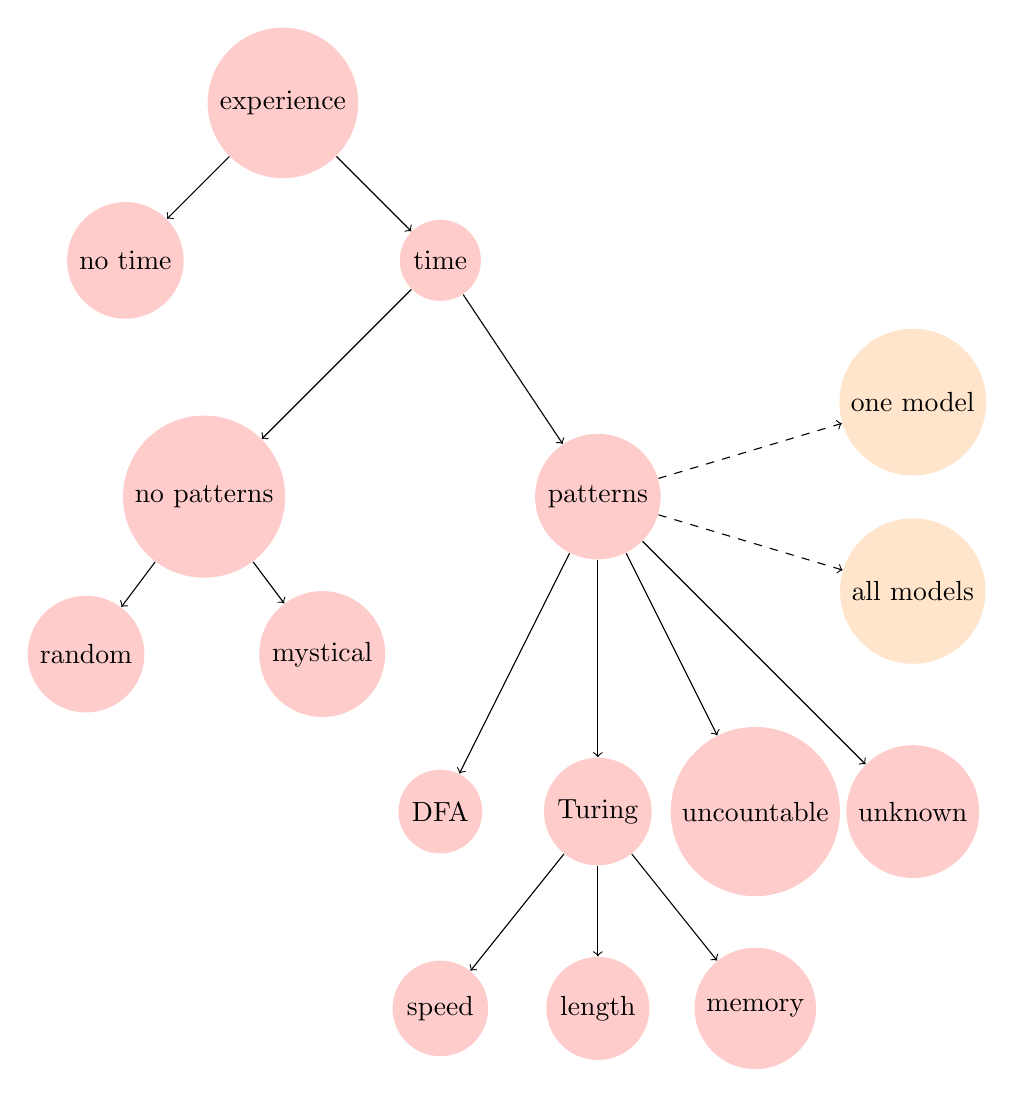
\begin{tikzpicture}
  		[scale=2,auto=left,every node/.style={circle,fill=red!20}]
  		\node (experience) at (4,3) {experience};
  		\node (notime) at (3,2) {no time};
  		\node (time) at (5,2) {time};
  		\node (nopatterns) at (3.5,0.5) {no patterns};
		\node (random) at (2.75, -0.5) {random};
		\node (mystical) at (4.25, -0.5) {mystical};
  		\node (patterns) at (6,0.5) {patterns};
		\node[fill=orange!20] (one) at (8,1.1) {one model};
		\node[fill=orange!20] (all) at (8,-0.1) {all models};
  		\node (dfa) at (5,-1.5) {DFA};
  		\node (turing) at (6,-1.5) {Turing};
  		\node (uncountable) at (7,-1.5) {uncountable};
  		\node (unknown) at (8,-1.5) {unknown};
		\node (speed) at (5,-2.75) {speed};
		\node (length) at (6,-2.75) {length};
		\node (memory) at (7,-2.75) {memory};
    	\foreach \from/\to in {
experience/notime,
experience/time,
time/patterns,
time/nopatterns,
patterns/dfa,
patterns/turing,
patterns/uncountable,
patterns/unknown,
turing/speed,
turing/length,
turing/memory,
nopatterns/random,
nopatterns/mystical}
    	\draw[->] (\from) -- (\to);
    	\foreach \from/\to in {
patterns/all,
patterns/one}
		\draw[dashed, ->] (\from) -- (\to);
	\end{tikzpicture}
}
\end{figure}

\newpage

\subsection{Impossible structures}

There is a language which can't be accpeted by any Turing machine, known as the \textit{diagonal language} $D = \{\langle M \rangle \mid \langle M \rangle \notin L_M \}$; where $L_M$ is a language which a machine $M$ accepts and $\langle M \rangle$ is a string encoding of $M$.
Language $D$ consists of string encodings of all machines which do not accept their own string encodings.\footnote
{
When you run a machine, you give it as input a string.
The machine will then either accept the string, reject the string, or enter an infinite loop.
The language of a machine is defined as the set of all the strings it accepts.
}
Does a machine $M_D$, a machine which accepts all strings in $D$, exist?
No, since if $M_D$ were to exist, that would imply that either:
\begin{enumerate}
\item $M_D$ accepts $\langle M_D \rangle$, which would imply that:
\begin{enumerate}
\item $\langle M_D \rangle \notin D$, since $D$ is defined as the set of string encodings of all machines which do not accept their own string encodings.
\item $\langle M_D \rangle \in D$, since $D$ is the set of all strings which $M_D$ accepts.
\end{enumerate}
\item $M_D$ does not accept $\langle M_D \rangle$, which would imply that:
\begin{enumerate}
\item $\langle M_D \rangle \in D$, since $D$ is defined as the set of string encodings of all machines which do not accept their own string encodings.
\item $\langle M_D \rangle \notin D$, since $D$ is the set of all strings which $M_D$ accepts.
\end{enumerate}
\end{enumerate}
Either way, there is a contradiction. This structure is \textit{defineable} yet it is \textit{impossible}.
There are some structures which are contradictory and can't exist.\footnote{Another famous one is the set of all sets that are not members of themselves, known as the Russell's paradox.}
Even those structures \textit{have properties}, or at least we can talk about the properties they would have if they were to be possible.
Us being capable to talk about them does not imply they are possible.

Are there structures which can't be described even by mathematics?
Such unknown unknowns can't be conclusively ruled out, but it remains unclear what to do about that possibility.

\newpage

\subsection{Uncountable structures}

There is a type of structure about which we can talk about, it has properties, is not contradictory, and can't be generated even with hypercomputation.
An example is the set of real numbers. 
Since the memory tape of the Turing machine is countable, there is no way for a machine to generate an uncountable data structure.
Even if we had some magic-Turing machine which could generate the set or reals, it could not iterate that set since a real number has no defined successor.\footnote{The rational numbers also have no successor.}
Going even further, imagine we had some super-magic-Turing machine which could iterate the set of reals, in that case it could print them in order, which would lead to a contradiction.

Each thought is a discrete entity and there is a limited number of them per unit of time.
How is it possible to talk about uncountable sets?
What we are doing when reasoning about uncountable sets is reasoning about properties.
The number of properties is countable, as is the number of axioms, and the number of steps in a proof.
If uncountable structures exist, then enumeration of all possible mathematical structures would be impossible, there would be no algorithm which can generate them.
Even if reality is something uncountable, we can at best approximate it with something countable.

\newpage

\subsection{Optimality}

The set of all Turing-complete programming languages is a one for which the invariance theorem holds.
It does not matter which member of the set we choose, because for all languages $A$ and $B$ and all strings $x$ there exists a constatnt $c$ such that $K_A(x) \leq K_B(x) + c$, as explained in the \textit{1.2.4 Invariance} subsection.
This is important since the goal is to have a method which assigns probability on the basis of the objects themselves, not based on the method used to describe them.
The invariance theorem does not hold in general for all description methods.
It is our conjecture that invariance holds only for Turing machines.

The other property which should hold is that of convergence.
Whatever the true process which generated the data is, algorithmic induction converges very fast to the true process, provided the process is computable.
It is our conjecture that no other choice of the prior converges faster.
Since our assumptions seem minimal, we claim this is the optimal theory of everything.

\newpage

\subsection{Solutions}

Here are some of the problems which are claimed to be solved:

\begin{itemize}
\item The problem of induction
\item The problem of solipsism
\item The problem of other minds
\item The problem of the fine-tuned universe
\item The problem of monism vs. dualism
\item The problem of something vs. nothing
\end{itemize}

\noindent
Some additional desiderata which are fulfilled:

\begin{itemize}
\item Is consistent with Epicurus' principle of multiple explanations
\item Is consistent with Bayes' theorem
\item Is a form of Occam's razor
\item Explains the invalidity of supernatural explanations
\item Explains the role of prediction and explanation in science
\item Dissolves the issue of refutability of scientific theories
\item Gives the definition of evidence
\item Gives the definition of explanatory power
\item Gives the definition of reality
\end{itemize}

\newpage

\subsection{Open problems}

\vspace{10px}

\begin{enumerate}
\item Indexicality in infinite structures depends in some unclear way on pattern recongition algorithms.
\item Observation selection problem.
\begin{enumerate}
\item Is there a general algorithm for proving if a set of rules is Turing-complete?
\end{enumerate}
\item Qualia is a type of knowledge of our internal mental states which is left to be explained. Task for some future chapter.
\item The demarcation problem in philosophy of science. Task for some future chapter.
\item If reality is a mathematical structure, why does time appear to flow? Task for our next chapter.
\end{enumerate}

\newpage

\subsection{Turning philosophy into math}

That which is in motion must arrive at the half-way point before it arrives at the goal.
Before it can get halfway there, it must get a quarter of the way there.
The resulting sequence can be represented as: $\{..., 1/16, 1/8, 1/4, 1/2\}$.
This requires one to complete an infinite number of tasks, which Zeno maintained is an impossibility.
Approximately a century after, Euclid did the work that shows that $\sum_{n=1}^{\infty} 2^{-n} = 1$.
This is an example of how philosophical problems can be turned into math, and solved.
As our knowledge keeps widening and deepening, at some time all philosophical problems shall be transmuted into math and solved.

\newpage
